\documentclass[11pt]{article}
\usepackage[margin=1in]{geometry}
\usepackage{amsmath,amssymb,booktabs,enumitem,float,graphicx,hyperref,xcolor}
\hypersetup{colorlinks=true,linkcolor=blue,urlcolor=blue,citecolor=blue}
\setlength{\emergencystretch}{3em}
\setlength{\parskip}{0.45em}
\setlength{\parindent}{0pt}
\newcommand{\E}{\mathbb E}
\newcommand{\R}{\mathbb R}
\title{Reinforcement Learning from Scratch\\\large Bellman Updates, Deep Q-Learning, and Self-Play}
\author{MATH 550 Course Module}
\date{August 15, 2026}

\begin{document}
\maketitle
\tableofcontents

\section{How to use this module}

This module is designed for four 75-minute meetings plus a computing lab.
Meeting 1 develops Markov decision processes, returns, value functions, and
tabular Q-learning. Meeting 2 turns the Bellman update into a PyTorch deep
Q-network (DQN) trained on MinAtar Breakout. Meeting 3 develops policy gradients,
actor-critic baselines, GAE, PPO, and the group-relative objective used by GRPO.
Meeting 4 introduces planning,
PUCT search, and AlphaZero-style self-play on Connect Four, then explains how
MuZero changes the known game model into a learned model. The lab runs the
reduced experiment first and then launches one full track.

After the module, students should be able to:
\begin{enumerate}[label=\arabic*.]
\item identify state, action, reward, termination, and discount conventions;
\item derive and implement one-step temporal-difference and Q-learning updates;
\item explain why replay and a target network stabilize DQN;
\item distinguish termination from a time limit and prevent an incorrect target;
\item derive the score-function estimator and explain how a baseline changes
variance but not its expectation;
\item implement GAE and PPO clipping, then interpret entropy, KL, clip fraction,
and explained variance;
\item distinguish PPO's environment actor-critic from outcome-supervision GRPO's
within-prompt group baseline;
\item implement PUCT selection, perspective-correct backup, and self-play labels;
\item explain why AlphaZero is not directly an Atari algorithm and how MuZero
learns a search model;
\item evaluate learning with held-out episodes, baselines, seeds, and uncertainty.
\end{enumerate}

\section{The reinforcement-learning problem}

A Markov decision process (MDP) is $(\mathcal S,\mathcal A,P,R,\gamma)$.
At time $t$, the agent sees $S_t=s$, selects $A_t=a$, receives $R_{t+1}$,
and moves to $S_{t+1}\sim P(\cdot\mid s,a)$. The Markov assumption says that
the current state contains the information needed to predict the next transition.
It does not say that the real world is memoryless; it says that the chosen state
representation is sufficient.

The discounted return is
\begin{equation}
G_t=R_{t+1}+\gamma R_{t+2}+\gamma^2R_{t+3}+\cdots,
\qquad 0\leq\gamma\leq1.
\end{equation}
The discount controls how rapidly delayed rewards lose weight and guarantees a
finite infinite-horizon sum when rewards are bounded and $\gamma<1$.

For policy $\pi(a\mid s)$,
\begin{align}
V^\pi(s)&=\E_\pi[G_t\mid S_t=s],\\
Q^\pi(s,a)&=\E_\pi[G_t\mid S_t=s,A_t=a].
\end{align}
Separating the first reward gives the Bellman expectation equation:
\begin{align}
Q^\pi(s,a)
&=\E\left[R_{t+1}+\gamma G_{t+1}\mid s,a\right]\\
&=\E\left[R_{t+1}+\gamma
\sum_{a'}\pi(a'\mid S_{t+1})Q^\pi(S_{t+1},a')\mid s,a\right].
\end{align}
Optimal action values instead satisfy
\begin{equation}
Q^*(s,a)=\E\left[R_{t+1}+\gamma\max_{a'}Q^*(S_{t+1},a')\mid s,a\right].
\end{equation}
This fixed-point equation is the source of the Q-learning target.

\section{From an equation to tabular Q-learning}

For one observed transition, replace the expectation with the sample target
\begin{equation}
Y_t=R_{t+1}+\gamma(1-D_{t+1})\max_{a'}Q(S_{t+1},a'),
\end{equation}
where $D_{t+1}=1$ for true termination. Then move the old value toward the target:
\begin{equation}
Q(S_t,A_t)\leftarrow Q(S_t,A_t)+\alpha\left[Y_t-Q(S_t,A_t)\right].
\end{equation}
The term in brackets is the temporal-difference error. Q-learning is off-policy:
the behavior may be $\epsilon$-greedy, while the target uses a greedy next action.

The course code in \texttt{gridworld.py} makes every quantity visible. A
$5\times5$ world has step reward $-0.04$, goal reward $+1$, pit reward $-1$,
and three walls. With seed 550, 1,500 episodes yield a final-100 mean return of
0.626 and an eight-step greedy path to the goal. This synthetic example isolates
the update before introducing neural approximation.

\subsection{Termination is not truncation}

If a transition ends because the task reached a terminal state, no future reward
exists and bootstrapping must stop. If a wrapper stops an otherwise continuing
task only because a time limit was reached, the mathematical state may still
have future value. Treating every time limit as terminal biases targets downward.
The MinAtar adapter records environment termination; the classroom step cap is
used to reset collection but is not inserted as a terminal replay label.

\section{Why deep Q-learning needs extra machinery}

Replace a table with a neural function $Q_\theta(s,a)$. A naive implementation
uses a moving network to define both prediction and target, trains on consecutive
highly correlated transitions, and revisits rare rewarding events only once.
These choices combine bootstrapping, function approximation, and off-policy data,
often called the ``deadly triad.'' DQN adds two practical controls.

\textbf{Experience replay.} Store transitions and sample them approximately
uniformly. This reuses data and weakens temporal correlation. The course replay
buffer is a fixed-capacity ring: observations remain \texttt{uint8}; only sampled
minibatches become floating-point tensors. The full 100,000-slot MinAtar buffer
allocates about 81.3 MB for current/next state, action, reward, and termination.

\textbf{Target network.} Hold parameters $\bar\theta$ fixed while optimizing
$\theta$, then periodically copy $\theta\to\bar\theta$. The target becomes less
mobile within an update block.

\subsection{DQN and Double-DQN targets}

Vanilla DQN uses
\begin{equation}
Y_t^{\mathrm{DQN}}=R_{t+1}+\gamma(1-D_{t+1})
\max_{a'}Q_{\bar\theta}(S_{t+1},a').
\end{equation}
The maximum chooses and evaluates with the same noisy estimates, which tends to
favor positive errors. Double-DQN separates the two roles:
\begin{align}
A^*&=\arg\max_{a'}Q_\theta(S_{t+1},a'),\\
Y_t^{\mathrm{Double}}&=R_{t+1}+\gamma(1-D_{t+1})
Q_{\bar\theta}(S_{t+1},A^*).
\end{align}
The code uses the Huber loss
\begin{equation}
\mathcal L(\theta)=\frac1B\sum_{i=1}^B
\operatorname{Huber}\left(Q_\theta(s_i,a_i)-y_i\right),
\end{equation}
which is quadratic near zero and linear for a large error. PyTorch supplies
convolutions, automatic differentiation, Adam, and gradient clipping; the RL
target and loop remain explicit.

\section{Atari at course scale}

The original DQN work learned from Atari pixels. Reproducing its multi-game
claims is not a few-hour classroom exercise. MinAtar instead supplies analogues
of Asterix, Breakout, Freeway, Seaquest, and Space Invaders on a $10\times10$
grid with object channels. This keeps the delayed-control problem while reducing
representational cost.

The primary class benchmark is MinAtar 1.0.15 Breakout from
\url{https://github.com/kenjyoung/MinAtar}, GPL-3.0. Its state has four binary
channels for game objects, and the module uses all six actions to match the
MinAtar paper. No pretrained model is loaded. The training data are the agent's
own transitions.

The repository includes a 50,000-transition random-policy dataset generated by
\begin{verbatim}
uv run --extra rl python -m experiments.reinforcement.collect_replay
\end{verbatim}
with an adjacent JSON provenance record. It is 0.78 MB compressed. The source
environment, version, seed, policy, tensor shapes, and license are recorded.

For a later raw-pixel extension, Farama provides
\texttt{atari/breakout/expert-v0}. Its authoritative page,
\url{https://minari.farama.org/main/datasets/atari/breakout/expert-v0/}, reports
23,075 transitions in 10 expert episodes, raw $210\times160\times3$ RGB frames,
and four actions. Download it exactly with
\begin{verbatim}
uv sync --locked --extra rl-data
uv run --extra rl-data minari download atari/breakout/expert-v0
\end{verbatim}
This optional data is not required by the compact online lab.

\section{Evaluation: learning is not a loss curve}

An RL loss is a changing regression problem. It can rise when the agent discovers
new high-return states and targets become larger. Evaluate policies in separate
episodes with learning disabled. Report score distributions, episode lengths,
hardware, environment version, action set, seeds, and wall time. A random policy
is the minimum baseline; a matched vanilla-DQN ablation is a useful extension.

The verified combined quick run used Apple M2 MPS. It performed 5,000 DQN
environment steps and 4,501 updates in 35.40 seconds (141.2 steps/s). Across six
evaluation
episodes, Double-DQN scored $3.33\pm0.21$ and random scored $0.67\pm0.33$.

\begin{figure}[h]
\centering
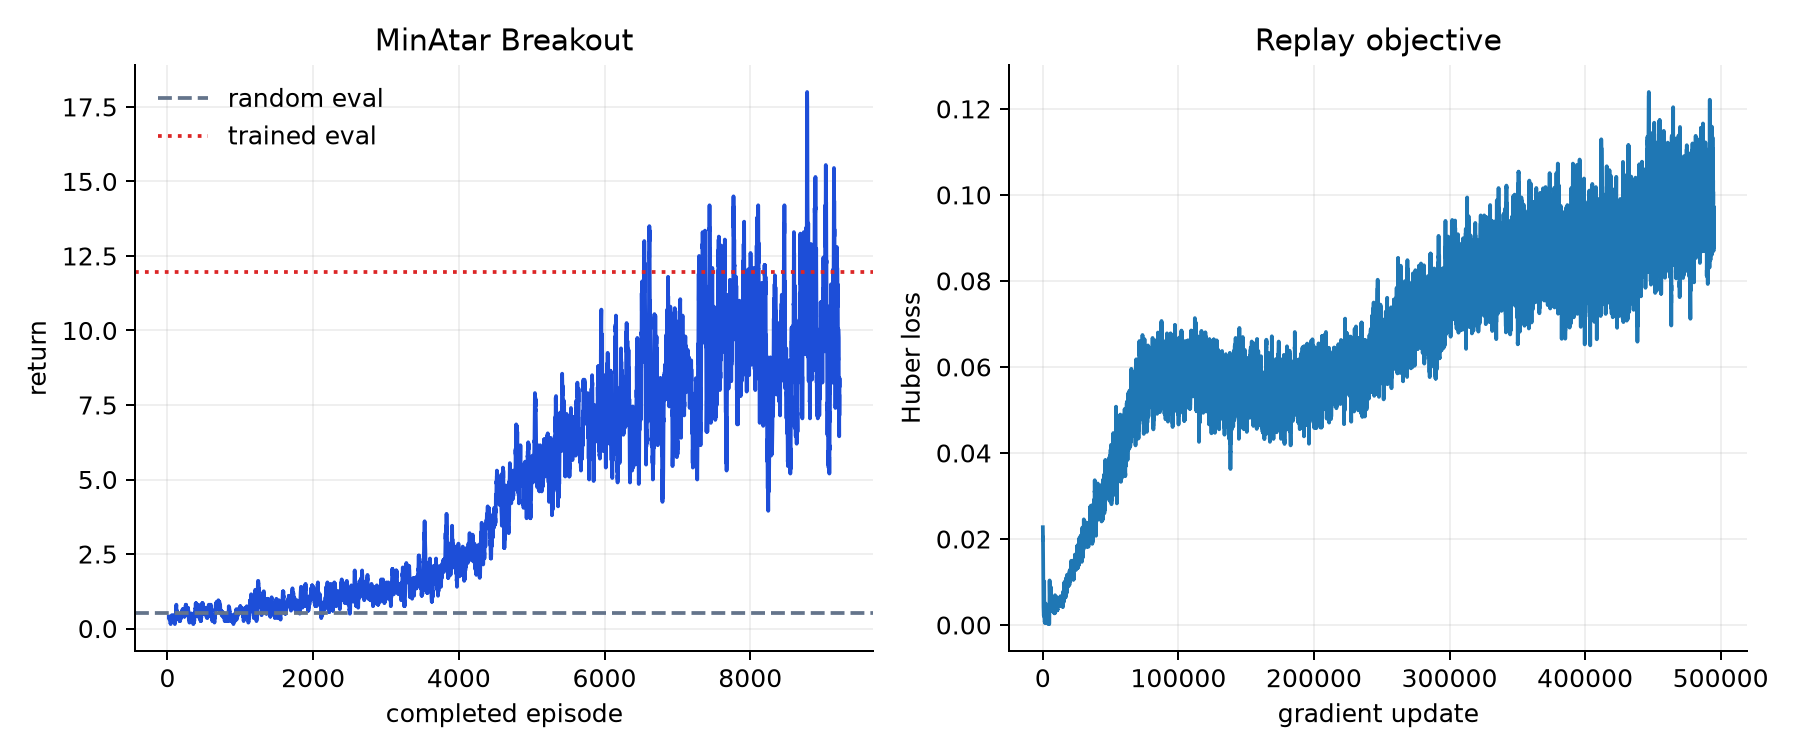
\includegraphics[width=\textwidth]{../../output/reinforcement/figures/dqn_training.png}
\caption{Measured quick-run data. A 5,000-step run verifies the pipeline but is
not a converged MinAtar benchmark.}
\end{figure}

At the measured throughput, 500,000 steps would take roughly 63 minutes if speed
scaled linearly. That extrapolation excludes evaluation, thermal effects, and
other workloads, so budget one to two hours on a comparable M2 and verify locally.
CUDA/Colab speeds vary. The correct unit of comparison is environment steps plus
the declared network/update schedule, not wall time alone.

\subsection{Inspect the learned policy, not only its score}

The playback demo loads a saved DQN or PPO checkpoint, runs one fixed-seed greedy
episode, and records the observation, selected action, immediate reward,
cumulative return, and full action-preference vector at every step. DQN frames
show raw $Q(s,a)$ values and a relative-preference bar; PPO frames show action
probabilities and the critic value $V(s)$. This makes a behavior claim
inspectable: students can check whether the paddle follows the ball and whether
the preferred action changes when the ball changes direction.

Run \texttt{make demo-reinforcement} after training. The command exports an
animated GIF, the contact sheet below, a CSV decision trace, and JSON provenance
with the checkpoint hash and environment seed. A single attractive trajectory
can be cherry-picked, so the playback supplements rather than replaces the
held-out evaluation distribution.

\begin{figure}[h]
\centering
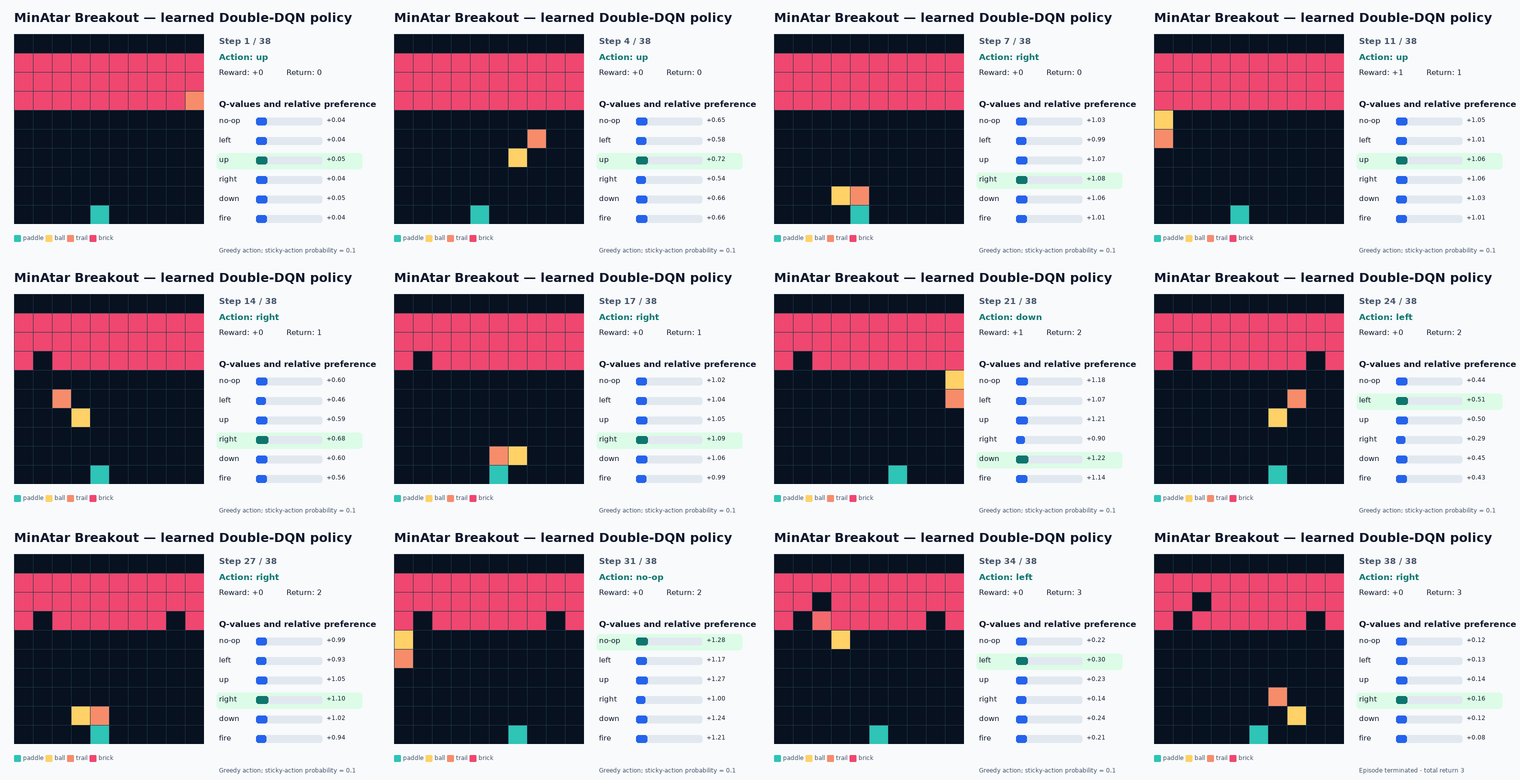
\includegraphics[width=\textwidth]{../../output/reinforcement/demos/minatar_breakout_dqn_learned_policy_contact_sheet.png}
\caption{Evenly sampled frames from one learned Double-DQN Breakout episode.
Every frame exposes the chosen action and all six learned action values.}
\end{figure}

\section{Policy gradients: optimize action probabilities directly}

DQN learns action values and takes an argmax. A policy-gradient method instead
parameterizes $\pi_\theta(a\mid s)$ and changes the probability of the action
actually sampled. For a trajectory return $G_t$, the likelihood-ratio identity
gives the REINFORCE estimator
\begin{equation}
\widehat{\nabla_\theta J}
=\frac1T\sum_{t=0}^{T-1}\nabla_\theta\log\pi_\theta(A_t\mid S_t)G_t.
\end{equation}
This form does not differentiate through the environment. In code, returns are
detached and gradient descent minimizes the negative expression. Reward-to-go
replaces a whole-episode return with rewards at and after time $t$, reducing
irrelevant noise.

\subsection{Deriving the score-function estimator rather than memorizing it}

For a finite trajectory $\tau$ with probability $p_\theta(\tau)$ and return
$R(\tau)$,
\begin{align}
J(\theta)&=\sum_\tau p_\theta(\tau)R(\tau),\\
\nabla_\theta J(\theta)
&=\sum_\tau p_\theta(\tau)R(\tau)\nabla_\theta\log p_\theta(\tau)\\
&=\E_{\tau\sim\pi_\theta}\left[R(\tau)
\sum_t\nabla_\theta\log\pi_\theta(A_t\mid S_t)\right].
\end{align}
The second line uses $\nabla p=p\nabla\log p$.  Environment transition
probabilities disappear from the derivative when they do not depend on
$\theta$.  This is why autograd follows selected-action log probabilities but
does not need a differentiable simulator.

The same derivation covers a language model.  The state is a prompt plus the
generated prefix, the action is the next token, and
\[
\log\pi_\theta(y\mid x)=\sum_{t=1}^{|y|}
\log\pi_\theta(y_t\mid x,y_{<t}).
\]
A terminal math verifier supplies $R(x,y)$.  This establishes the conceptual
bridge from this RL module to the following reasoning module; it does not make
GRPO an appropriate algorithm for every control problem.

\subsection{Why a baseline is unbiased---and why ``mean reward'' is not always optimal}

For any baseline $b(s)$ that does not depend on the sampled action,
\begin{align}
\E_{A\sim\pi_\theta}[b(s)\nabla_\theta\log\pi_\theta(A\mid s)]
&=b(s)\sum_a\pi_\theta(a\mid s)\nabla_\theta\log\pi_\theta(a\mid s)\\
&=b(s)\nabla_\theta\sum_a\pi_\theta(a\mid s)=0.
\end{align}
Thus subtraction preserves the expectation, but its variance depends on the
score-vector magnitude.  A complete binary example makes the distinction
visible.  Let $A\sim\mathrm{Bernoulli}(p)$, $p=\sigma(\theta)$, and $R=A$.
Since $\partial_\theta\log\pi_\theta(A)=A-p$, one sample with baseline $b$ is
\[
Z_b=(A-b)(A-p)=
\begin{cases}(1-b)(1-p),&A=1,\\bp,&A=0.\end{cases}
\]
Its mean is always $p(1-p)$ and the variance of an average of $n$ samples is
\[
\operatorname{Var}(\bar Z_b)=\frac1n\left[
p(1-b)^2(1-p)^2+(1-p)b^2p^2-p^2(1-p)^2\right].
\]
With no baseline this becomes $p(1-p)^3/n$.  With the population reward mean
$b=p$, it becomes $p(1-p)(1-2p)^2/n$: lower for $p<2/3$, equal at $p=2/3$,
and higher for $p>2/3$.  The variance-minimizing scalar is instead $b^*=1-p$
in this special example, producing zero variance.  The lesson is precise:
valid baselines preserve the target gradient; they do not automatically reduce
variance.

Subtracting a state-only baseline preserves the estimator's expectation because
$\sum_a\pi_\theta(a\mid s)\nabla_\theta\log\pi_\theta(a\mid s)=0$. A learned
critic $V_\phi(s)$ therefore changes variance, not the optimum. Its residual is
\begin{equation}
\delta_t=R_{t+1}+\gamma(1-D_{t+1})V_\phi(S_{t+1})-V_\phi(S_t).
\end{equation}
Generalized advantage estimation trades bias against variance:
\begin{equation}
\hat A_t^{\mathrm{GAE}(\gamma,\lambda)}
=\delta_t+(\gamma\lambda)(1-D_{t+1})\delta_{t+1}+\cdots.
\end{equation}
At $\lambda=0$ this is a one-step residual. Near $\lambda=1$ it approaches a
Monte Carlo-style advantage. The terminal mask prevents residuals from leaking
across reset episodes.

\subsection{PPO is token/action-level importance reweighting}

PPO is easiest to understand as a controlled reuse of a fresh rollout.  At
iteration $k$, freeze a behavior policy $\pi_{\rm old}=\pi_{\theta_k}$,
collect states and actions from it, and store every selected-action log
probability.  During optimization the live parameters become $\theta$, so
each sampled action receives the ratio

Let
\begin{equation}
r_t(\theta)=\exp\left(
\log\pi_\theta(A_t\mid S_t)-\log\pi_{\theta_{\rm old}}(A_t\mid S_t)
\right).
\end{equation}
The old log probability is stored during rollout collection. PPO's clipped
surrogate is
\begin{equation}
L^{\rm clip}(\theta)=\E_t\left[
\min\left(r_t(\theta)\hat A_t,
\operatorname{clip}(r_t(\theta),1-\epsilon,1+\epsilon)\hat A_t\right)
\right].
\end{equation}
Before clipping, differentiate one surrogate term:
\begin{equation}
\nabla_\theta\{r_t(\theta)\hat A_t\}
=r_t(\theta)\hat A_t\nabla_\theta
\log\pi_\theta(A_t\mid S_t).
\end{equation}
Thus PPO is still a policy gradient.  The difference from on-policy REINFORCE
is the token/action-specific coefficient $r_t\hat A_t$.  The ratio is not a
loss weight applied after differentiation: because $\nabla r_t=r_t\nabla
\log\pi_\theta$, it is exactly the multiplier on the sampled score gradient.

The pessimistic minimum creates a signed saturation rule.  Away from the two
boundaries, the coefficient multiplying the score gradient under gradient
ascent is
\begin{equation}
c_t(\theta)=
\begin{cases}
0,&\hat A_t>0\ \text{and}\ r_t>1+\epsilon,\\
0,&\hat A_t<0\ \text{and}\ r_t<1-\epsilon,\\
r_t\hat A_t,&\text{otherwise}.
\end{cases}
\end{equation}
A positive-advantage action saturates only after becoming too much more likely.
A negative-advantage action saturates only after becoming too much less likely.
The other two outside-window cases remain live because their gradient moves the
policy back toward the desired direction.  This is why ``ratio outside the
window'' and ``clipping removed the gradient'' are different diagnostics.

\subsection{Why language-model PPO is token-level}

For an autoregressive model, $S_t=(x,y_{<t})$ and $A_t=y_t$.  One response has
\[
\rho_t(\theta)=\frac{\pi_\theta(y_t\mid x,y_{<t})}
{\pi_{\rm old}(y_t\mid x,y_{<t})}.
\]
Even when a terminal verifier produces one response-level advantage $\hat A$,
the token ratios differ because every prefix defines a different conditional
distribution.  PPO therefore applies
\[
\sum_{t=1}^{|y|}\min\{\rho_t\hat A,
\operatorname{clip}(\rho_t,1-\epsilon,1+\epsilon)\hat A\},
\]
possibly with a token or sequence normalization.  Outcome supervision assigns
the same sign to all sampled response tokens; PPO's ratios change their
magnitudes and saturation states, but do not reveal which reasoning step was
causally correct.  A critic, generalized advantage estimation, process reward,
or another credit mechanism is needed for genuinely different token advantages.

The exact importance ratio for the whole sampled response is instead
\begin{equation}
\rho_{\rm seq}(y\mid x)=\frac{\pi_\theta(y\mid x)}
{\pi_{\rm old}(y\mid x)}=\prod_{t=1}^{|y|}\rho_t(\theta).
\end{equation}
Replacing this product by separately clipped token terms is not exact sequence
importance sampling.  It is a lower-variance, biased surrogate that treats the
sampled old-policy prefixes as fixed training contexts.

\begin{figure}[H]
\centering
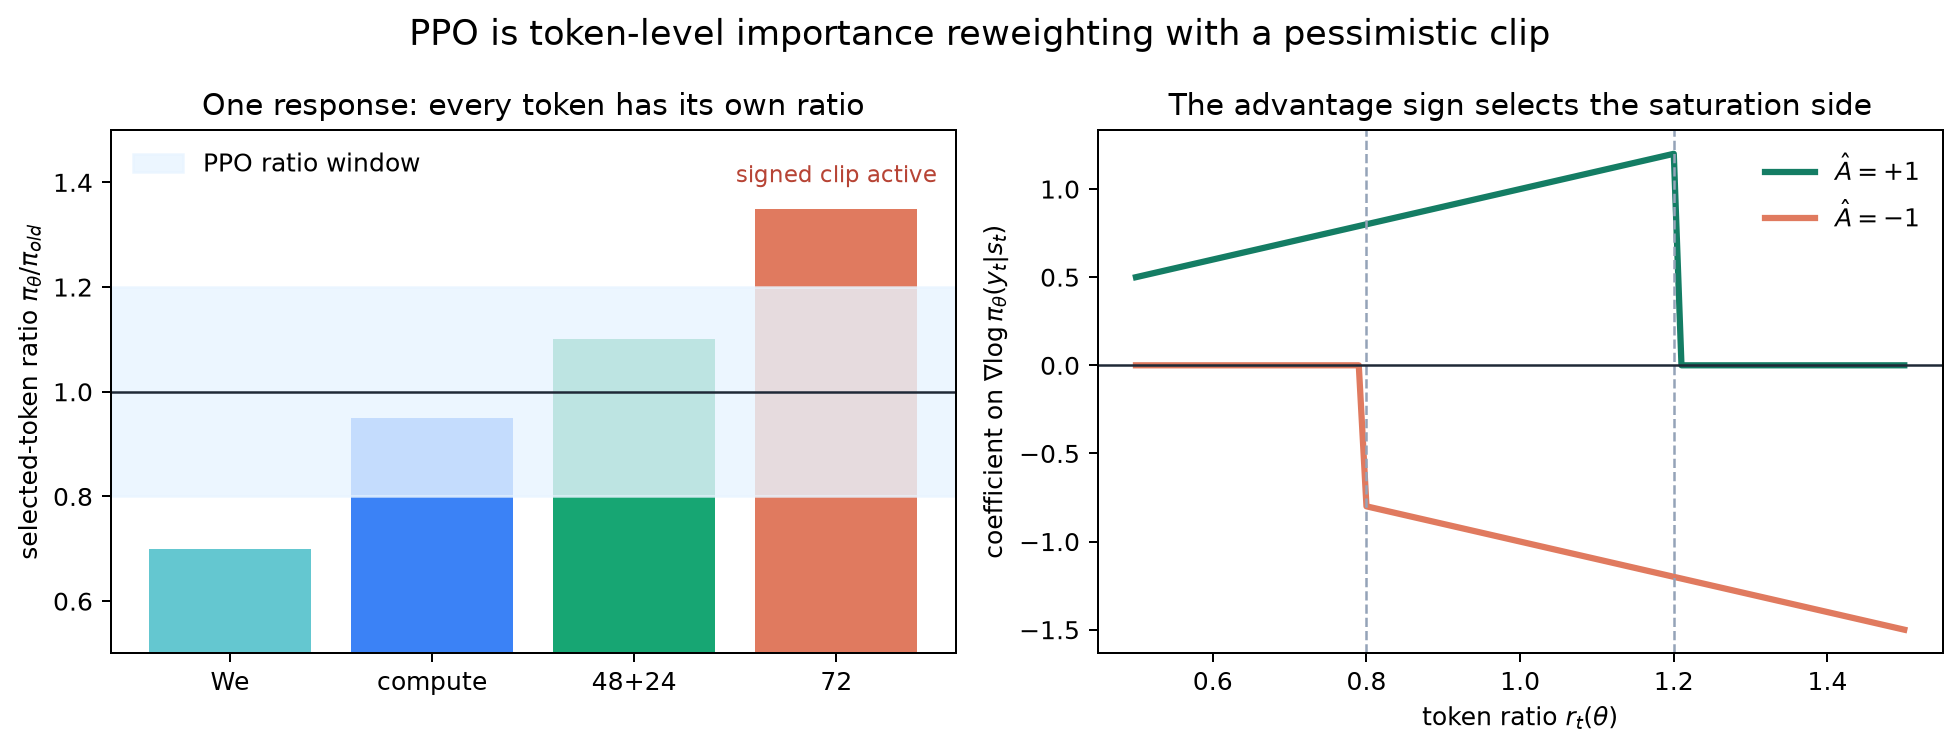
\includegraphics[width=\textwidth]{../../output/reinforcement/figures/ppo_token_reweighting.png}
\caption{Deterministic tensor audit.  The left panel uses one positive-advantage
response: every selected token has its own old-to-new ratio, and only the last
token enters the signed saturation region.  The right panel plots the exact
coefficient on each score gradient.  This figure demonstrates estimator
mechanics, not learned-policy quality.}
\end{figure}

\subsection{PPO is near-on-policy, not fully on-policy or replay-buffer off-policy}

The data are on-policy at collection time: the first update begins with
$\theta=\theta_{\rm old}$ and every ratio is one.  PPO then performs several
minibatch epochs without recollecting data.  After the first optimizer step,
the same actions and prefixes are stale samples from $\pi_{\rm old}$; the
ratios acknowledge that limited off-policy reuse.

This does not make PPO a general off-policy algorithm like DQN.  The action
ratio corrects $\pi_\theta(a\mid s)/\pi_{\rm old}(a\mid s)$ at sampled old-policy
states, but the state-visitation distribution is still $d^{\pi_{\rm old}}$, not
$d^{\pi_\theta}$.  Clipping deliberately biases even the action correction.
PPO therefore alternates
\[
\text{fresh rollout from }\pi_{\rm old}
\longrightarrow\text{a few corrected/clipped epochs}
\longrightarrow\text{discard rollout and recollect}.
\]
Target KL, clip fraction, active-clip fraction, and mean ratio reveal when the
``few nearby epochs'' approximation is breaking.  A fixed reference policy in
RLHF is separate: $\pi_{\rm old}$ records who generated the data, whereas
$\pi_{\rm ref}$ regularizes behavior drift.

Clipping is not a proof that the whole policy is close.  It only flattens the
sampled surrogate in two signed regions, so the implementation also logs
approximate KL and both outside-window and active clipping fractions.

The course actor-critic shares a convolutional trunk and has a categorical
policy head plus a scalar value head. Eight MinAtar environments collect a
$128\times8$ rollout. Course code computes terminal-masked GAE, normalizes the
advantages, shuffles minibatches, performs a small number of epochs, clips value
changes and gradient norm, adds entropy, and optionally stops early on KL. No
RL trainer or rollout library is called.

The verified 8,192-step PPO track in that combined MPS run took 3.55 seconds and
completed 64 minibatch updates. Six held-out deterministic episodes scored $0.83\pm0.17$,
while six uniform-random episodes scored $0.50\pm0.34$. Final approximate KL was
0.0011, clip fraction 0.0, entropy 1.769, and explained variance 0.295. These
small samples validate mechanics and instrumentation, not PPO superiority.

\begin{figure}[h]
\centering
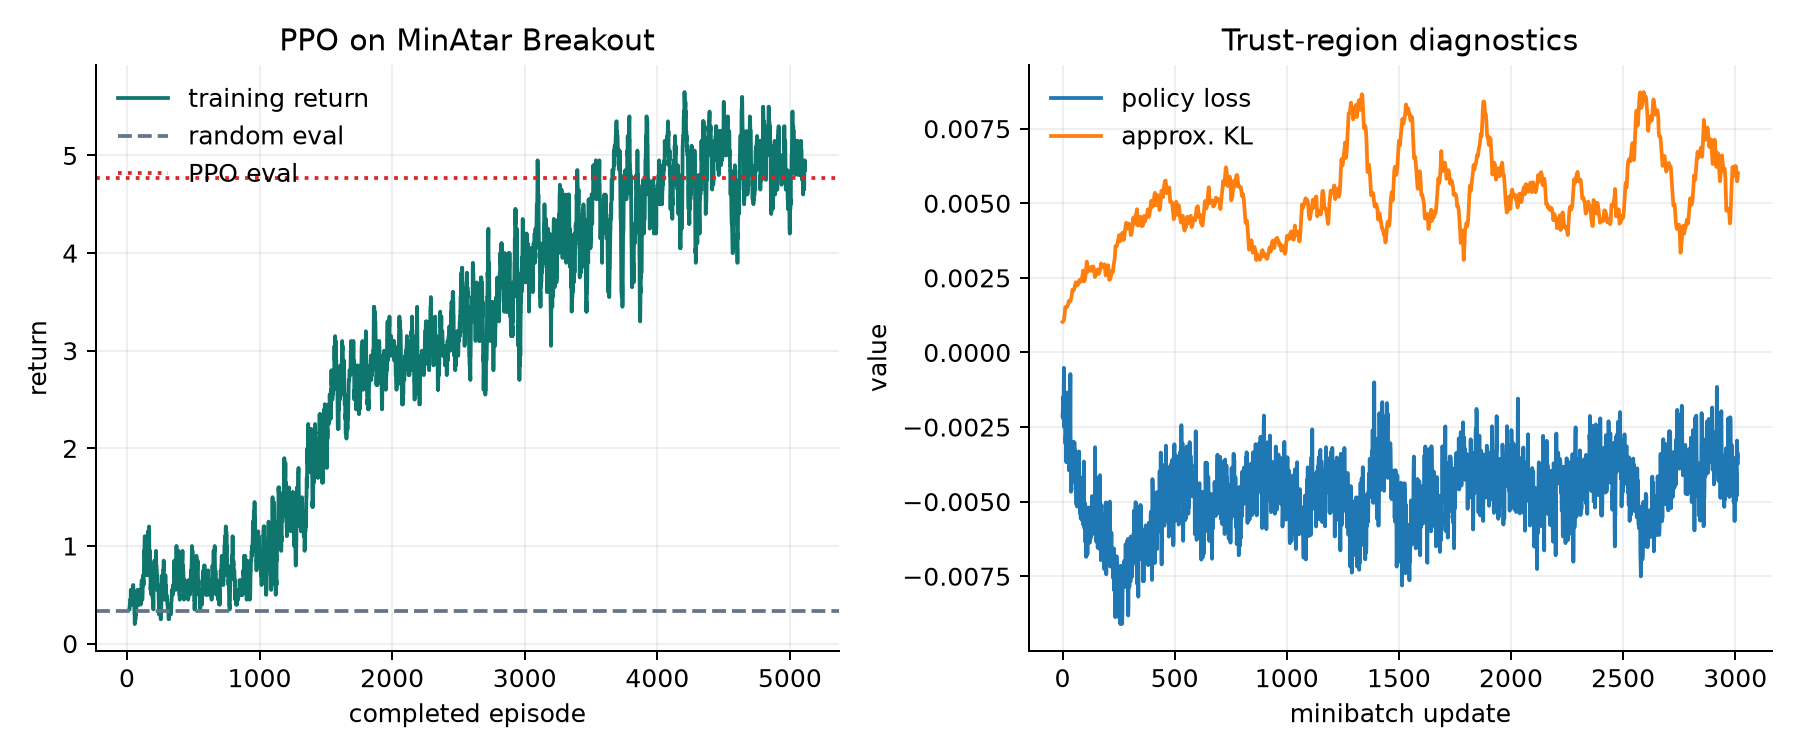
\includegraphics[width=\textwidth]{../../output/reinforcement/figures/policy_gradient_training.png}
\caption{PPO smoke-run returns and update diagnostics. A short, one-seed run is
not a convergence study.}
\end{figure}

\subsection{GRPO replaces the critic with a within-prompt comparison}

The original DeepSeekMath outcome-supervision GRPO construction samples a group
of $G$ completions for the same prompt and standardizes their scalar rewards:
\begin{equation}
\hat A_i=\frac{R_i-\operatorname{mean}(R_1,\ldots,R_G)}
{\operatorname{std}(R_1,\ldots,R_G)+\varepsilon}.
\end{equation}
It then uses a PPO-style clipped likelihood ratio and a penalty relative to a
reference policy. The positive per-token KL estimator used in this module is
\begin{equation}
\exp\left(\log\pi_{\rm ref}-\log\pi_\theta\right)
-\left(\log\pi_{\rm ref}-\log\pi_\theta\right)-1\geq0.
\end{equation}
Group normalization provides a baseline without a value network, but it needs
multiple meaningfully different scored samples for one prompt. If every reward
ties, every advantage is zero. PPO on MinAtar and GRPO on grouped completions
therefore share clipping machinery but solve differently structured problems;
GRPO is not a drop-in replacement for Atari PPO.

For $G$ independent responses to one prompt, the empirical group mean
$\bar R=G^{-1}\sum_jR_j$ depends on all sampled responses.  It is therefore not
the ordinary action-independent baseline above.  Expanding the diagonal and
cross terms gives
\[
\E\left[\frac1G\sum_{j=1}^{G}(R_j-\bar R)
\nabla\log\pi_\theta(Y_j\mid x)\right]
=\frac{G-1}{G}\nabla J_x(\theta).
\]
The direction is preserved up to a finite-$G$ scale, but this fact should be
stated rather than hidden behind the word ``baseline.''  Dividing by the group
standard deviation changes the expectation again and reweights prompts by
difficulty.  The reasoning module treats baseline, advantage scaling, token
importance correction, clipping, and loss normalization as separate switches.

\subsection{Exact stale-rollout correction explains PPO's approximation}

If rollouts came from $\pi_0$ but the current policy is $\pi_\theta$, the naive
score-function estimator is biased.  Exact sequence importance sampling uses
\[
w(y\mid x)=\frac{\pi_\theta(y\mid x)}{\pi_0(y\mid x)}
=\prod_t\frac{\pi_\theta(y_t\mid x,y_{<t})}
{\pi_0(y_t\mid x,y_{<t})}.
\]
It corrects the sequence probability under a fixed prompt, but its variance can
grow exponentially with sequence length.  A fully changed state/prompt
distribution would require additional occupancy correction.  PPO/GRPO token
clipping, CISPO upper clipping, and GSPO's geometric-mean sequence ratio are
biased variance-control choices.  Clipping a ratio does not make stale data
on-policy; it changes how stale-data bias and variance are managed.

\section{Planning and self-play}

Value-based control chooses actions with a learned value function. Search instead
uses a simulator to compare possible futures before acting. In a deterministic
two-player zero-sum game such as Connect Four, each node records a prior $P$, visit
count $N$, and mean action value $Q$. PUCT selects
\begin{equation}
a^*=\arg\max_a\left[Q(s,a)+c_{\mathrm{puct}}P(s,a)
\frac{\sqrt{N(s)+1}}{N(s,a)+1}\right].
\end{equation}
Selection descends the tree. Expansion asks the network for legal-action priors
and a leaf value. Backup updates every node on the path, reversing the sign when
the player perspective changes.

The sign reversal is easy to get wrong. The network value at state $s$ is from
the current player's perspective. If a child state belongs to the opponent, a
value favorable to that child is unfavorable to its parent. The tests create a
known four-in-a-row position and check outcomes from both perspectives.

\subsection{AlphaZero-style training targets}

The network $f_\theta(s)=(p_\theta,v_\theta)$ shares a residual trunk. The policy
head returns seven column logits. The value head returns a scalar in $[-1,1]$.
For each self-play position, the normalized root visit counts produce $\pi$.
After the game ends, the winner produces $z$ from the player-at-that-position's
perspective. Horizontal reflection is an exact Connect Four symmetry and doubles
the data.

The joint objective is
\begin{equation}
\mathcal L=-\pi^\top\log p_\theta(s)+(z-v_\theta(s))^2
+\lambda\lVert\theta\rVert_2^2.
\end{equation}
The loop alternates search-generated data and minibatch training. No expert games
or pretrained policy are used.

\begin{figure}[h]
\centering
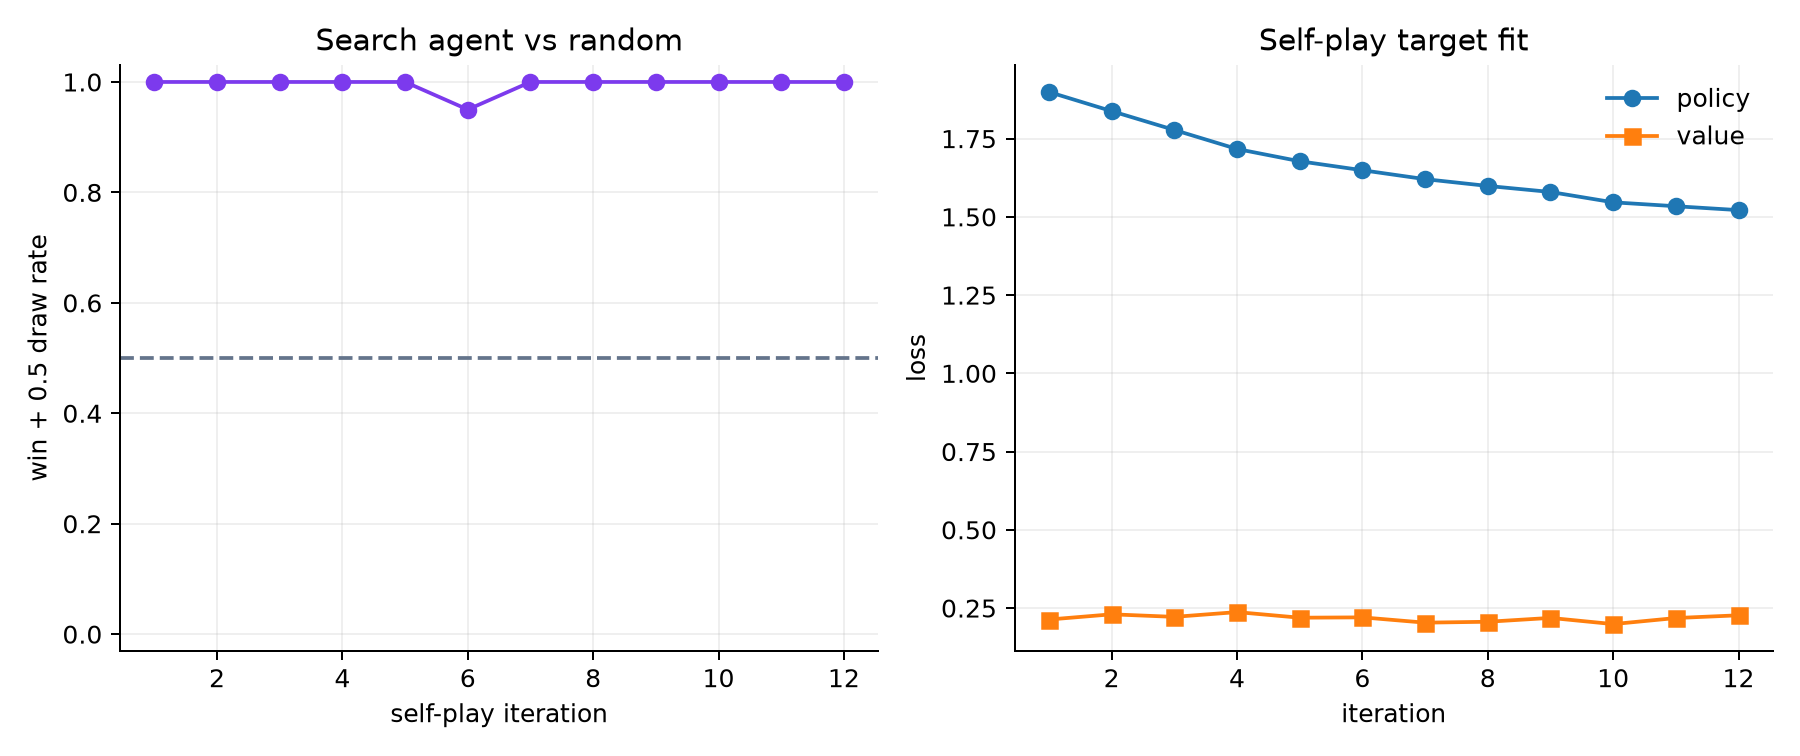
\includegraphics[width=\textwidth]{../../output/reinforcement/figures/alpha_zero_self_play.png}
\caption{One quick self-play iteration. The arena contains only four games;
the score is a software check, not statistical evidence of improvement.}
\end{figure}

The smoke run generated 78 reflection-augmented positions from three games.
Its four-game arena score against random was 1.0 before and after training. This
illustrates why a baseline can be too weak and an arena too small. A stronger
course experiment should use more iterations, 50 or more arena games, several
seeds, and a checkpoint league or previous-network comparison.

\section{Why AlphaZero is not the Atari model}

AlphaZero receives the game rules through the simulator used by MCTS. Connect
Four has two alternating players, deterministic transitions, known legal moves,
and a terminal win/draw/loss. Atari is single-agent, visually complex, and has
unknown dynamics from the agent's viewpoint. Calling DQN experience collection
``self-play'' would be incorrect; there is no second copy of the policy as an
opponent.

MuZero keeps search but learns the model needed by search. In compact notation:
\begin{align}
s^0&=h_\theta(o_{1:t}) && \text{representation},\\
(r^{k+1},s^{k+1})&=g_\theta(s^k,a^{k+1}) && \text{dynamics},\\
(p^k,v^k)&=f_\theta(s^k) && \text{prediction}.
\end{align}
The learned state need not reconstruct pixels; it needs to predict rewards,
values, and policies useful for planning. Training unrolls actions from replay
and compares predicted rewards, policies, and values with observed rewards and
search/bootstrap targets. Atari data comes from the current agent interacting
with the environment, while planning occurs in the learned latent dynamics.

This course implements the full AlphaZero mechanics on Connect Four and uses DQN
for the Atari track. A faithful MuZero implementation is a valuable capstone but
adds representation/dynamics networks, value and reward supports, recurrent
unrolls, replay reanalysis, and more expensive search. Those additions should be
visible and tested rather than hidden behind a library.

\section{Implementation map}

\begin{tabular}{p{0.31\textwidth}p{0.62\textwidth}}
\toprule
File & Teaching responsibility \\
\midrule
\texttt{gridworld.py} & MDP transitions, epsilon-greedy action, Q update \\
\texttt{replay.py} & fixed-capacity byte ring and uniform sampling \\
\texttt{models/dqn.py} & convolutional Q network, Double-DQN target, explicit loop \\
\texttt{policy\_gradient.py} & REINFORCE/GAE/PPO/GRPO losses, actor-critic, explicit PPO loop \\
\texttt{connect\_four.py} & legal moves, terminal logic, perspective encoding \\
\texttt{alpha\_zero.py} & policy/value network, PUCT, backup, self-play, joint loss \\
\texttt{run\_benchmark.py} & configuration, held-out evaluation, artifacts \\
\texttt{test\_reinforcement.py} & equations, shapes, rules, devices, public environment \\
\bottomrule
\end{tabular}

\section{Commands and run plans}

\begin{verbatim}
uv sync --locked --extra rl
make test-reinforcement
make quick-reinforcement
make audit-rlvr  # shared estimator audit used by the next module

# Full few-hour teaching tracks (run separately if desired)
uv run --extra rl python -m experiments.reinforcement.run_benchmark \
  --device auto --track dqn
uv run --extra rl python -m experiments.reinforcement.run_benchmark \
  --device auto --track ppo
uv run --extra rl python -m experiments.reinforcement.run_benchmark \
  --device auto --track selfplay
\end{verbatim}

On Colab, clone the repository, install \texttt{uv}, run the same sync command,
and use \texttt{--device cuda}. On Apple Silicon use \texttt{--device mps} or
\texttt{auto}. An explicit unavailable accelerator raises an error instead of
silently falling back.

\section{Failure modes and diagnostics}

\begin{itemize}
\item \textbf{High or noisy loss:} inspect evaluation return and target scale;
loss alone does not measure policy quality.
\item \textbf{No reward:} verify actions, termination, reward logging, and
epsilon decay before changing architecture.
\item \textbf{Optimistic Q values:} compare vanilla and Double-DQN targets;
track chosen Q values alongside returns.
\item \textbf{PPO appears frozen:} inspect reward frequency, entropy, advantage
scale, approximate KL, and clip fraction before increasing the epoch count.
\item \textbf{PPO jumps too far:} lower the learning rate or epoch count and use
the target-KL stop; clipping alone does not enforce a hard trust region.
\item \textbf{GRPO has zero gradient:} check whether all rewards within each
prompt group tie or whether a token mask removed every valid token.
\item \textbf{MCTS illegal action:} mask before normalization and test a full column.
\item \textbf{Wrong self-play values:} attach each terminal label to the player
stored with that position and reverse perspective during backup.
\item \textbf{MPS/CUDA mismatch:} move both network and every tensor to the same
resolved device. A CPU-only test is insufficient for this failure.
\item \textbf{False improvement:} alternate colors, increase arena size, use
multiple seeds, and compare against stronger checkpoints.
\end{itemize}

\section{References}

\begin{enumerate}
\item R. Sutton and A. Barto, \emph{Reinforcement Learning: An Introduction},
2nd ed., 2018, \url{http://incompleteideas.net/book/the-book-2nd.html}.
\item V. Mnih et al., ``Human-level control through deep reinforcement
learning,'' \emph{Nature} 518, 2015,
\url{https://doi.org/10.1038/nature14236}.
\item K. Young and T. Tian, ``MinAtar: An Atari-Inspired Testbed for Thorough
and Reproducible Reinforcement Learning Experiments,'' 2019,
\url{https://arxiv.org/abs/1903.03176}.
\item R. Williams, ``Simple Statistical Gradient-Following Algorithms for
Connectionist Reinforcement Learning,'' 1992,
\url{https://doi.org/10.1007/BF00992696}.
\item J. Schulman et al., ``High-Dimensional Continuous Control Using
Generalized Advantage Estimation,'' 2015, \url{https://arxiv.org/abs/1506.02438}.
\item J. Schulman et al., ``Proximal Policy Optimization Algorithms,'' 2017,
\url{https://arxiv.org/abs/1707.06347}.
\item L. Ouyang et al., ``Training Language Models to Follow Instructions with
Human Feedback,'' 2022, \url{https://arxiv.org/abs/2203.02155}.
\item Z. Shao et al., ``DeepSeekMath: Pushing the Limits of Mathematical
Reasoning in Open Language Models,'' 2024, \url{https://arxiv.org/abs/2402.03300}.
\item Stanford CS336, ``Assignment 5: Alignment,'' Spring 2026,
\url{https://github.com/stanford-cs336/assignment5-alignment}.  The reviewed
course copy matches repository revision \texttt{c2734a2} byte for byte.
\item Z. Liu et al., ``Understanding R1-Zero-Like Training: A Critical
Perspective,'' 2025, \url{https://arxiv.org/abs/2503.20783}.
\item F. Tajwar et al., ``Maximum Likelihood Reinforcement Learning,'' 2026,
\url{https://arxiv.org/abs/2602.02710}.
\item C. Zheng et al., ``Group Sequence Policy Optimization,'' 2025,
\url{https://arxiv.org/abs/2507.18071}.
\item D. Silver et al., ``Mastering Chess and Shogi by Self-Play with a General
Reinforcement Learning Algorithm,'' 2017,
\url{https://arxiv.org/abs/1712.01815}.
\item J. Schrittwieser et al., ``Mastering Atari, Go, Chess and Shogi by Planning
with a Learned Model,'' 2019, \url{https://arxiv.org/abs/1911.08265}.
\item Farama Foundation, \href{https://minari.farama.org/main/datasets/atari/breakout/expert-v0/}
{Minari Breakout expert dataset documentation}.
\end{enumerate}

\end{document}
